\documentclass[11pt]{article}

\usepackage[margin=1in]{geometry}
\usepackage{amsmath,amssymb,mathtools}
\usepackage{microtype}
\usepackage{xcolor}
\usepackage{tikz}
\usetikzlibrary{arrows.meta,positioning,calc}
\usepackage{hyperref}

\hypersetup{
  colorlinks=true,
  linkcolor=blue!55!black,
  citecolor=blue!55!black,
  urlcolor=blue!55!black,
}

\setlength{\parindent}{0pt}
\setlength{\parskip}{0.55em}
\numberwithin{equation}{section}

\newcommand{\R}{\mathbb{R}}
\newcommand{\softmax}{\operatorname{softmax}}

\title{Flash Attention}
\author{Haowu Duan}
\date{\today}

\begin{document}

\maketitle

\begin{abstract}
This note develops FlashAttention from ordinary scaled dot-product
attention.  The central question is how to compute exact attention while reducing
data movement between GPU memory and on-chip memory.
\end{abstract}

\tableofcontents
\newpage

\section{The problem FlashAttention solves}

For a sequence of length $N$ and a head dimension $d$, let
$Q,K,V\in\R^{N\times d}$.  Scaled dot-product attention is
\begin{equation}
  O
  = \softmax\!\left(\frac{QK^{\mathsf T}}{\sqrt d}\right)V,
  \qquad O\in\R^{N\times d},
  \label{eq:standard-attention}
\end{equation}
where softmax is applied independently to each row.

A direct implementation materializes the $N\times N$ score matrix and usually the
$N\times N$ probability matrix in high-bandwidth memory.  FlashAttention computes
the same mathematical result without materializing either full matrix.  It divides
$Q$, $K$, and $V$ into tiles, moves one collection of tiles into fast on-chip
memory, and incrementally combines partial softmax results.  The algorithm changes
the order of computation and memory access, not the definition in
Equation~\eqref{eq:standard-attention}.

The key technical step is an online softmax update.  It lets a row of attention be
normalized correctly even when its logits arrive one tile at a time.  The next
section will derive that update before mapping it to GPU tiles.

\newpage
\section{The four FlashAttention algorithms}

The first version establishes the tiled online-softmax algorithm.  Each later
version addresses a performance bottleneck exposed by a newer kernel design or GPU
generation.

Split the query sequence into row tiles $Q_i\in\R^{B_r\times d}$ and split the key
and value sequences into column tiles
$K_j,V_j\in\R^{B_c\times d}$.  The indices $i$ and $j$ label query and key--value
tiles.  A causal or padding mask is represented by the tile
$M_{ij}\in(\R\cup\{-\infty\})^{B_r\times B_c}$.  Within a tile,
$r\in\{1,\ldots,B_r\}$ labels a query row, $c\in\{1,\ldots,B_c\}$ labels a
key--value row, and $a\in\{1,\ldots,d\}$ labels a head component.  Masked or
out-of-range positions have $(M_{ij})_{rc}=-\infty$.

Figure~\ref{fig:flashattention-tile-dataflow} shows one iteration.  A thread block
keeps one query tile and its running state on chip while it visits key--value tiles
from left to right.  Only the shaded $B_r\times B_c$ score tile exists during the
iteration.

\begin{figure}[htbp]
  \centering
  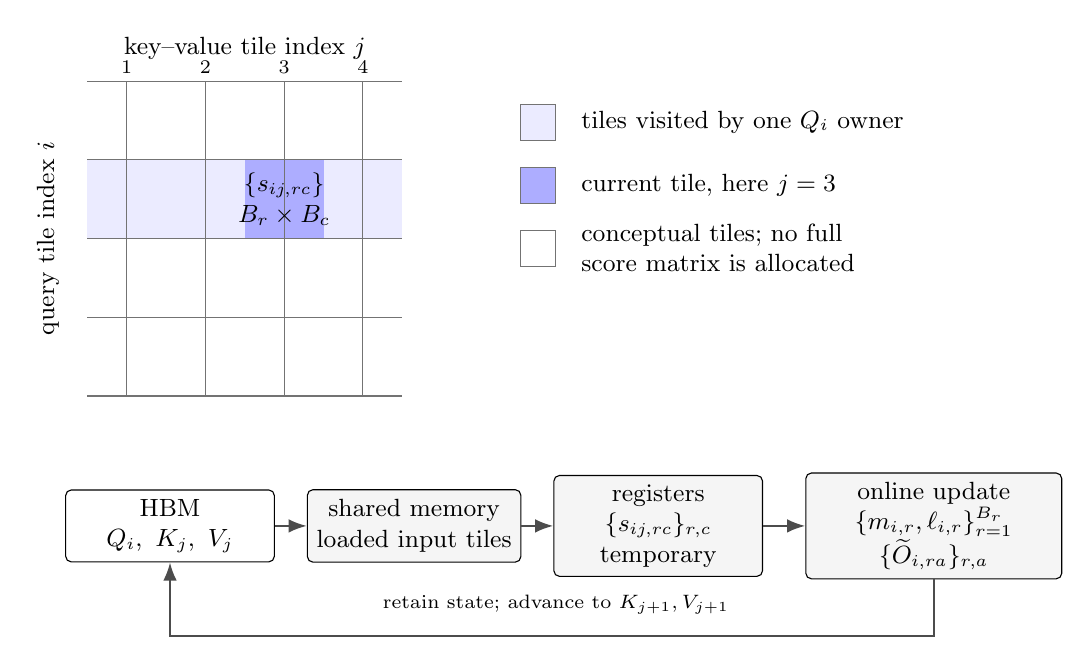
\begin{tikzpicture}[
    font=\small,
    >=Latex,
    memory/.style={draw,rounded corners=2pt,minimum width=2.65cm,
      minimum height=0.82cm,align=center},
    operation/.style={draw,rounded corners=2pt,fill=black!4,
      minimum width=2.65cm,minimum height=0.92cm,align=center},
    flow/.style={->,thick,black!70}
  ]
    % A 4-by-4 grid of score tiles.  The second tile row is owned by Q_i,
    % and the third tile in that row is the current (i,j) tile.
    \fill[blue!8] (0.5,5.0) rectangle (4.5,6.0);
    \fill[blue!32] (2.5,5.0) rectangle (3.5,6.0);
    \draw[step=1cm,black!55] (0.5,3.0) grid (4.5,7.0);
    \node at (2.5,7.42) {key--value tile index $j$};
    \node[rotate=90] at (0.0,5.0) {query tile index $i$};
    \node[align=center] at (3.0,5.5)
      {$\{s_{ij,rc}\}$\\$B_r\times B_c$};
    \foreach \x/\lab in {1/1,2/2,3/3,4/4}
      \node[font=\scriptsize] at (\x,7.18) {$\lab$};

    \fill[blue!8] (6.0,6.25) rectangle (6.45,6.70);
    \draw[black!55] (6.0,6.25) rectangle (6.45,6.70);
    \node[anchor=west] at (6.65,6.48)
      {tiles visited by one $Q_i$ owner};
    \fill[blue!32] (6.0,5.45) rectangle (6.45,5.90);
    \draw[black!55] (6.0,5.45) rectangle (6.45,5.90);
    \node[anchor=west] at (6.65,5.68)
      {current tile, here $j=3$};
    \draw[black!55] (6.0,4.65) rectangle (6.45,5.10);
    \node[anchor=west,align=left] at (6.65,4.88)
      {conceptual tiles; no full\\score matrix is allocated};

    \node[memory] (hbm) at (1.55,1.35)
      {HBM\\$Q_i,\ K_j,\ V_j$};
    \node[operation] (sram) at (4.65,1.35)
      {shared memory\\loaded input tiles};
    \node[operation] (score) at (7.75,1.35)
      {registers\\$\{s_{ij,rc}\}_{r,c}$\\temporary};
    \node[operation,minimum width=3.25cm] (state) at (11.25,1.35)
      {online update\\
       $\{m_{i,r},\ell_{i,r}\}_{r=1}^{B_r}$\\
       $\{\widetilde O_{i,ra}\}_{r,a}$};

    \draw[flow] (hbm) -- (sram);
    \draw[flow] (sram) -- (score);
    \draw[flow] (score) -- (state);
    \draw[flow] (state.south) -- ++(0,-0.72) -| (hbm.south);
    \node[font=\scriptsize,fill=white,inner sep=1pt] at (6.45,0.35)
      {retain state; advance to $K_{j+1},V_{j+1}$};
  \end{tikzpicture}
  \caption{One FlashAttention tile iteration.  The grid represents the conceptual
  $N\times N$ score matrix, partitioned into tiles.  The kernel creates only the
  highlighted tile, incorporates it into the running state, discards it, and moves
  to the next key--value tile.}
  \label{fig:flashattention-tile-dataflow}
\end{figure}

\subsection{FlashAttention-1: tiled exact attention}
\label{sec:fa1}

FlashAttention-1 makes exact attention I/O-aware.  It loads tiles into on-chip
static random-access memory (SRAM), forms a score tile, and immediately consumes
that tile.  The complete $N\times N$ score and probability matrices are never
written to high-bandwidth memory (HBM)~\cite{dao2022flashattention}.

For every row $r$ of query tile $i$, initialize the running maximum
$m_{i,r}$, running denominator $\ell_{i,r}$, and every component of the
normalized output $O_{i,ra}$ by
\begin{equation}
  m_{i,r}^{(0)}=-\infty,
  \qquad \ell_{i,r}^{(0)}=0,
  \qquad O_{i,ra}^{(0)}=0,
  \qquad
  \substack{1\le r\le B_r\\1\le a\le d}.
  \label{eq:fa1-initial-state}
\end{equation}
When key--value tile $j$ arrives, first compute every score in its
$B_r\times B_c$ score tile and the largest score in each query row:
\begin{align}
  s_{ij,rc}
  &=\frac{1}{\sqrt d}\sum_{a=1}^{d}
      (Q_i)_{ra}(K_j)_{ca}+(M_{ij})_{rc},
  &\widehat m_{ij,r}
  &=\max_{1\le c\le B_c}s_{ij,rc},
  \label{eq:fa1-score}\\
  \widehat p_{ij,rc}
  &=\exp\!\left(s_{ij,rc}-\widehat m_{ij,r}\right),
  &\widehat\ell_{ij,r}
  &=\sum_{c=1}^{B_c}\widehat p_{ij,rc}.
  \label{eq:fa1-local-softmax}\\
  m_{i,r}^{(j)}
  &=\max\!\left(m_{i,r}^{(j-1)},\widehat m_{ij,r}\right),
  \label{eq:fa1-new-maximum}\\
  \ell_{i,r}^{(j)}
  &=e^{m_{i,r}^{(j-1)}-m_{i,r}^{(j)}}\ell_{i,r}^{(j-1)}
    +e^{\widehat m_{ij,r}-m_{i,r}^{(j)}}\widehat\ell_{ij,r}.
  \label{eq:fa1-new-denominator}
\end{align}
Subtracting a row maximum keeps every exponential argument non-positive.  When a
new tile has a larger maximum, the two exponential factors convert the old and
new partial sums to the common reference value $m_{i,r}^{(j)}$.

FlashAttention-1 keeps every output component normalized after each tile:
\begin{align}
  O_{i,ra}^{(j)}
  =\frac{1}{\ell_{i,r}^{(j)}}\Biggl[
    &e^{m_{i,r}^{(j-1)}-m_{i,r}^{(j)}}
      \ell_{i,r}^{(j-1)}O_{i,ra}^{(j-1)}
  \nonumber\\
    &+e^{\widehat m_{ij,r}-m_{i,r}^{(j)}}
      \sum_{c=1}^{B_c}\widehat p_{ij,rc}(V_j)_{ca}
  \Biggr],
  \qquad
  \substack{1\le r\le B_r\\1\le a\le d}.
  \label{eq:fa1-output-update}
\end{align}
After the last key--value tile, $O_i^{(T_c)}$ equals the corresponding rows of
Equation~\eqref{eq:standard-attention}, where $T_c=\lceil N/B_c\rceil$.

The forward kernel follows this order:
\begin{enumerate}
  \item Load a $K_j,V_j$ tile from HBM into SRAM.
  \item For every compatible query tile $Q_i$, form the scores
        $\{s_{ij,rc}\}_{r,c}$ and apply
        Equations~\eqref{eq:fa1-local-softmax}--\eqref{eq:fa1-output-update}.
  \item Write the updated $O_{i,ra}^{(j)},m_{i,r}^{(j)},\ell_{i,r}^{(j)}$ state to
        HBM and continue with the next key--value tile.
\end{enumerate}
The backward kernel reloads $Q$, $K$, and $V$ tiles and recomputes the local score
and probability tiles needed for the derivatives.  Recomputation adds arithmetic
but avoids saving an $N\times N$ probability matrix during the forward pass.  This
is the central memory tradeoff in FlashAttention-1.

\subsection{FlashAttention-2: better accumulation and work partitioning}
\label{sec:fa2}

FlashAttention-2 retains tiling and online softmax but removes repeated
normalization of the output accumulator.  It stores an unnormalized numerator
$\widetilde O_{i,ra}$ until the query tile has visited every key--value tile
\cite{dao2023flashattention2}.  Initialize
\begin{equation}
  m_{i,r}^{(0)}=-\infty,
  \qquad \ell_{i,r}^{(0)}=0,
  \qquad \widetilde O_{i,ra}^{(0)}=0.
\end{equation}
For tile $j$, compute $s_{ij,rc}$ as in Equation~\eqref{eq:fa1-score}, then update
\begin{align}
  m_{i,r}^{(j)}
  &=\max\!\left(m_{i,r}^{(j-1)},
                \max_{1\le c\le B_c}s_{ij,rc}\right),
  &p_{ij,rc}
  &=\exp\!\left(s_{ij,rc}-m_{i,r}^{(j)}\right),
  \label{eq:fa2-score-update}\\
  \ell_{i,r}^{(j)}
  &=e^{m_{i,r}^{(j-1)}-m_{i,r}^{(j)}}\ell_{i,r}^{(j-1)}
    +\sum_{c=1}^{B_c}p_{ij,rc},
  \label{eq:fa2-denominator-update}\\
  \widetilde O_{i,ra}^{(j)}
  &=e^{m_{i,r}^{(j-1)}-m_{i,r}^{(j)}}\widetilde O_{i,ra}^{(j-1)}
    +\sum_{c=1}^{B_c}p_{ij,rc}(V_j)_{ca}.
  \label{eq:fa2-numerator-update}
\end{align}
Only after the final tile does the kernel normalize and save the log-sum-exp state:
\begin{equation}
  O_{i,ra}
  =\frac{\widetilde O_{i,ra}^{(T_c)}}{\ell_{i,r}^{(T_c)}},
  \qquad
  L_{i,r}=m_{i,r}^{(T_c)}+\log\ell_{i,r}^{(T_c)}.
  \label{eq:fa2-finalize}
\end{equation}
Delaying normalization performs fewer non-matrix-multiplication operations because
the full $B_r\times d$ output tile is not divided after every key--value tile.

FlashAttention-2 also changes which GPU workers own the tiles:
\begin{enumerate}
  \item Parallelize over query tiles in addition to batch elements and heads.  One
        thread block owns one query tile and scans the required $K_j,V_j$ tiles.
  \item Split $Q_i$ across warps while making $K_j,V_j$ available to those warps.
        Each warp produces its own output rows, which avoids the shared-memory
        reduction required by the split-$K$ arrangement in FlashAttention-1.
  \item In the backward pass, parallelize over key--value column tiles and combine
        contributions to $dQ$ as required.
\end{enumerate}
These changes target occupancy and shared-memory traffic.

\subsection{FlashAttention-3}
\label{sec:fa3}
\subsection{FlashAttention-4}
\label{sec:fa4}

This two subsections are intentionally left for later.  FlashAttention-3 and -4 are specific to
newer hardware, so I will write them after gaining hands-on experience with the
corresponding GPUs.  I currently work mostly with NVIDIA A800 and RTX 3090 GPUs.


\begin{thebibliography}{9}

\bibitem{dao2022flashattention}
Tri Dao, Daniel Y. Fu, Stefano Ermon, Atri Rudra, and Christopher R\'e.
\newblock FlashAttention: Fast and memory-efficient exact attention with
I/O-awareness.
\newblock In \emph{Advances in Neural Information Processing Systems}, 2022.
\newblock \url{https://arxiv.org/abs/2205.14135}.

\bibitem{dao2023flashattention2}
Tri Dao.
\newblock FlashAttention-2: Faster attention with better parallelism and work
partitioning.
\newblock In \emph{International Conference on Learning Representations}, 2024.
\newblock \url{https://arxiv.org/abs/2307.08691}.

\end{thebibliography}

\end{document}
